\section{Analysis}
\label{sec:analysis}

\subsection{Error taxonomy}

Figure~\ref{fig:error-hist} reports the distribution of evaluator error types
per model. Three patterns are worth flagging.

\begin{figure}[!htbp]
  \centering
  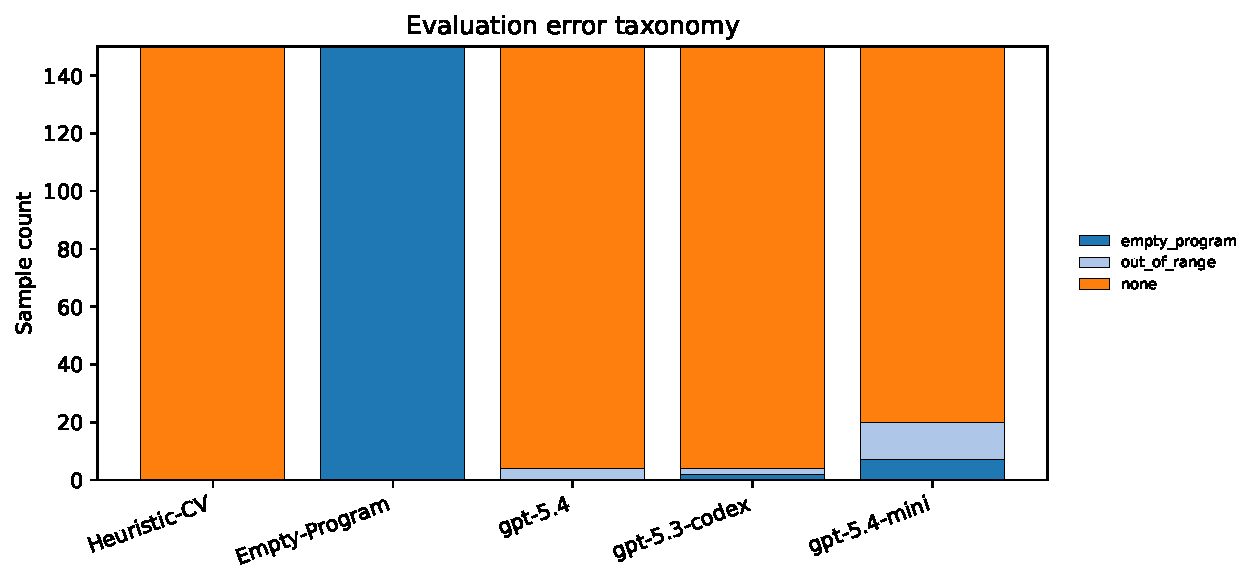
\includegraphics[width=\linewidth]{figures/fig_error_histogram.pdf}
  \caption{Evaluator error taxonomy per model. The ``none'' bar counts samples
  whose predictions parsed and rendered without error, including samples that
  did not pixel-match the target. Remaining categories surface structured
  parsing or validation failures.}
  \label{fig:error-hist}
\end{figure}

First, \texttt{Empty-Program} concentrates all 150 samples under the
\texttt{empty\_program} parse error, because an empty DSL program is a parse
failure by construction. This is the intended floor and not a pathology.

Second, the LLM runs have non-zero but small parse-failure counts, dominated by
\texttt{out\_of\_range} (predicted coordinates or extents outside the valid
$[0,511]$ and $[1, 512]$ ranges) and \texttt{invalid\_stroke} (stroke widths
exceeding the primitive's documented limit). These are cases where the model
understood the task format but violated structural constraints -- the kind of
failure mode that shows models do not internalize the DSL's range constraints
from a short prompt alone.

Third, the \texttt{Heuristic-CV} baseline has \emph{zero} parse failures because
it only emits programs it can itself construct. Its errors manifest as low
foreground IoU rather than parse failures.

\subsection{Qualitative wins and losses}

Figure~\ref{fig:qualitative} shows representative wins (top rows) and losses
(bottom rows) for the best exact-match multimodal configuration: each row shows
the target image, the prediction rendered through the same renderer, and the XOR
diff of foreground masks. The wins are dominated by the easy tier, where two or
three
non-overlapping shapes can be located and parameterized precisely. Losses tend
to come from medium and hard tiers and split into three recurring categories:
(i) correct shape inventory but off-by-a-few-pixel parameter estimates, (ii)
missed occluded shapes in high-overlap hard scenes, and (iii) misclassification
of hollow vs. filled when stroke widths are thin.

\begin{figure}[!htbp]
  \centering
  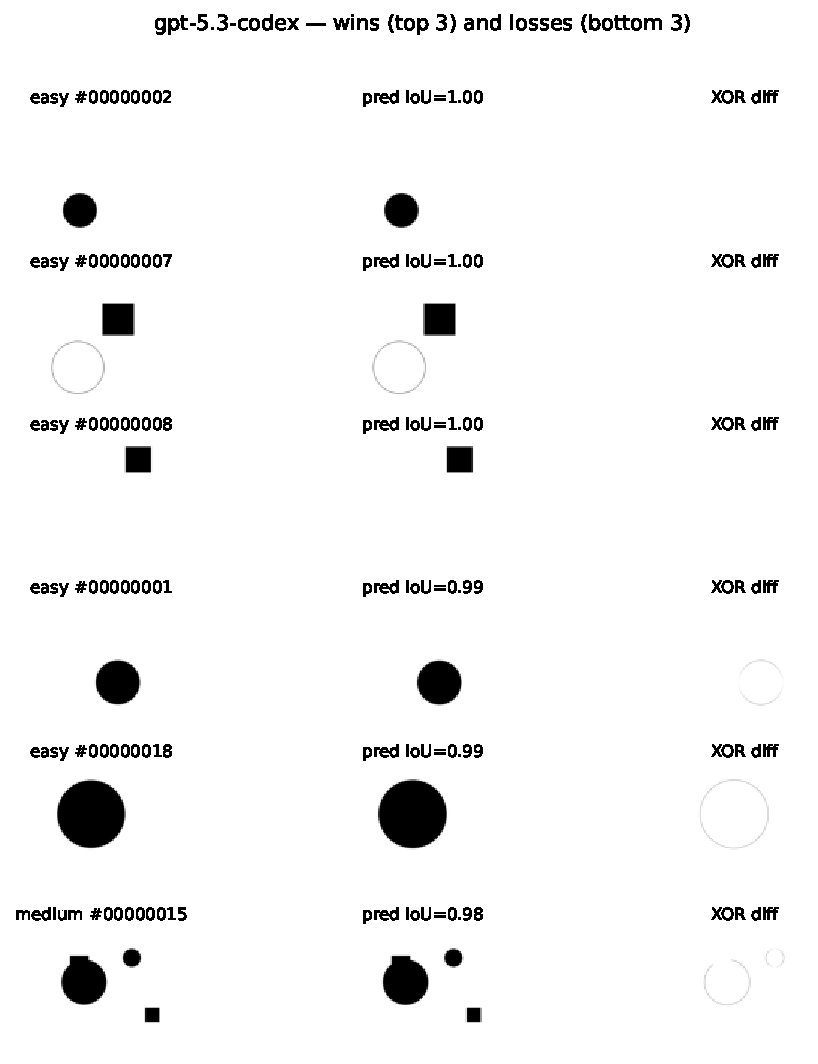
\includegraphics[width=0.95\linewidth]{figures/fig_qualitative_grid.pdf}
  \caption{Wins (top) and losses (bottom) for the best exact-match multimodal
  configuration on \textsc{eval\_v1} (\textsc{GPT-5.5} at \texttt{medium}
  reasoning effort, selected automatically by exact-match rate). Each row shows
  the target, the re-rendered prediction, and a foreground-XOR diff. Losses
  cluster on overlapping hard scenes and stroke-width confusions.}
  \label{fig:qualitative}
\end{figure}

\subsection{Difficulty validity}

A renewable benchmark is useful only if its difficulty tiers track real
performance gradients. Figure~\ref{fig:acc-by-diff} shows that exact-match rate
falls monotonically from easy to hard for every system, including the heuristic
baseline. Foreground IoU tracks the same ordering but with shallower slopes, as
expected: pixel-level similarity degrades more gracefully than the all-or-nothing
exact-match metric. This monotonic structure supports the claim that
\textsc{eval\_v1}'s difficulty axes are not arbitrary.

\subsection{Heuristic vs. LLM gap}

The heuristic baseline anchors what a purely bottom-up computer-vision pipeline
with no DSL-level reasoning can achieve. Its story splits by tier. On the easy
tier it is surprisingly competitive on \emph{exact-match}, because easy scenes
are separated and unclipped -- connected components match shapes directly, the
area/perimeter stroke estimator is close enough, and the hollow-vs-filled test
on eroded masks rarely errs. Multimodal models, by contrast, almost always
miss exact-match on easy scenes by a few pixels of parameter error: they
recover the \emph{right shapes} but not the \emph{right parameter values}.

On the medium and hard tiers the picture flips. Foreground IoU for the
heuristic deteriorates sharply because overlapping or clipped shapes merge
into a single connected component and the pipeline can no longer individuate
them. Multimodal models retain most of the spatial structure (foreground IoU
stays roughly flat across tiers) but still do not pixel-match -- their
programs contain the right number of shapes in roughly the right positions,
but they cannot land parameters precisely under occlusion.

Taken together, the heuristic is a better \emph{exact-match} baseline on easy
scenes and a worse \emph{IoU} baseline on harder ones. This decomposition is
precisely the kind of diagnostic signal \textsc{ShapeCodeBench} is designed to
produce: difficulty is not a single-axis phenomenon, and different systems
fail in different places. The sharp easy-tier exact-match comparison also
argues that closing that gap -- having a model emit \emph{both} the right
shape list \emph{and} the right parameter values on clean scenes -- is a
natural first-order target for future work.
